\documentclass[a4paper,12pt,twoside]{report}
\usepackage[left=2cm,right=2cm,top=2cm,bottom=3cm]{geometry}
\usepackage[spanish]{babel}
\usepackage[utf8]{inputenc}
\usepackage{svg}
\usepackage{xcolor}
\usepackage{graphicx}
\usepackage{float}
\usepackage{listings}
\usepackage{tipa}
\usepackage{lscape} 


\usepackage{xcolor}
\usepackage{soul}
\newcommand{\macb}{\textcolor{red}}

\graphicspath{ {./imagenes/} }

\title{Anotación automática de un corpus hablado de licencia abierta y larga duración para el lenguaje Español}
\author{Mauricio Collazos}
\date{March 2021}

\begin{document}

\maketitle

\begin{abstract}
    Los recursos abiertos para el procesamiento, reconocimiento, generación y demás tareas relacionadas con las tecnologías del lenguaje hablado son parte fundamental del proceso académico e investigativo. Estos recursos deben contener características muy específicas para la ejecución adecuada de la tarea relacionada, donde los niveles de anotación, duración de las grabaciones, variedad de locutores, balance de género, tamaño del vocabulario, relación de señal/ruido y conjunto de datos para pruebas son fundamentales. A pesar de existir diversos recursos disponibles para realizar las tareas mencionadas, los recursos abiertos para trabajar las tecnologías del hablada en la lengua española son escasos y en muchos casos insuficientes para realizar comparaciones con investigaciones del estado del arte propuestas para otros lenguajes. Este trabajo realiza una exploración de los recursos abiertos para el español y propone mecanismos para segmentar audio libros publicados por voluntarios bajo licencias abiertas en recursos apropiados para el procesamiento de voz.
\end{abstract}


\chapter{Introducción}

\section{Definición del problema}

Los recursos para la investigación de tecnologías del habla son de vital importancia para la generación y validación de nuevo conocimiento en el área. En la actualidad donde la investigación se ha decantado en su mayoría por el aprendizaje de máquina utilizando mecanismos de aprendizaje supervisado, semi supervisado y no supervisado \cite{Chiu2018} \cite{AmazonSemiSupervised}  \cite{ZeroResources} , la calidad de los datos usados para el entrenamiento, validación y pruebas definen en gran medida los resultados de la investigación.

Recursos representativos para realizar tareas comunes como el reconocimiento automático del habla y la síntesis del habla son TIMIT \cite{PriceTheRecognition}, Switchboard \cite{Godfrey1992SWITCHBOARD:Development}, Fisher \cite{CieriTheSpeech-to-Text} y Libri Speech \cite{PanayotovLIBRISPEECH:BOOKS}, recursos anotados desde el nivel fonético hasta el nivel de declaración altamente citados en investigaciones relacionadas con tecnologías del habla para la lengua inglesa


Aunque se ha probado el uso de recursos multilingues para tareas de reconocimiento de voz, la diferenciación en la articulación de los fonemas hace necesaria el uso de recursos enfocados en el español. \macb{Cu\'ales son los recursos multilingues? es sólo la fonolog\'ia lo que hace \'util tener recursos en espa\~nol?}

Para la lengua española, los recursos más representativos para realizar tareas relacionadas con procesamiento de voz son Albazyn \cite{CampilloAlbayzinEvaluation}, Fisher Spanish \cite{FischerSpa}, Call Friend \cite{CALLFRIENDSpa}, Call Home \cite{CALLHOMESpa}, DIMEx100\cite{Pineda2004DIMEx100:Spanish}, y mas recientemente Libri Speech español \cite{LibriVox-Spanish}.



El presente trabajo realiza una revisión detallada \macb{de} recursos abiertos para la ejecución de tareas de voz y propone la creación \macb{de} un nuevo recurso basado en grabaciones accesibles en la web de licencias abiertas\macb{\st{, utilizando}. Para ello se emplea} algoritmos de segmentación y alineamiento para la anotación a nivel de sentencia de un corpus de larga duración, gran vocabulario y de múltiples locutores.


\section{Justificación}


Existen múltiples factores importantes que influyen en los resultados de investigación con tareas de voz como el nivel de anotación de los recursos, la relación ruido señal, la variación de locutores, y el tamaño del vocabulario\macb{\st{, pero}. Sin embargo, } se ha mostrado que el tamaño del corpus es un factor que impacta directamente la precisión de las tareas. \macb{D\'nde se ha demostrado? Cu\'ales son los estudios, o estudios que muestren este efecto?. Citar ejemplos}

En la tabla \ref{tab:english_corpora} se presentan recursos representativos para la lengua inglesa, siendo estos corpus objeto de múltiples investigaciones. \macb{Sugiero que si no se tiene el n\'umero de palabras del vocabulario, es mejor retirar esa columna.}

\begin{table}[H]
\centering
\caption{Corpus hablados en la lengua inglesa\macb{. La duraci\'on est\'a en horas.}}
% \caption{Speech English Corpus}
\label{tab:english_corpora}
\begin{tabular}{|l|l|l|l|l|}
\textbf{Base de datos} & \textbf{Duración} & \textbf{Vocabulario} & \textbf{Anotación} & \textbf{Licencia}\\
\hline
FISHER\cite{CieriTheSpeech-to-Text}  & más de 2000 & Muy grande &  Declaración & LDC Non-Members\\
\hline
LIBRISPEECH\cite{PanayotovLIBRISPEECH:BOOKS}  & más de 1000 & Muy grande &  Declaración & CC BY 4.0\\
\hline

Switchboard \cite{Godfrey1992SWITCHBOARD:Development}  & 240 & Muy grande & Palabras & LDC Non-Members\\
\hline
\multicolumn{1}{|p{3.4cm}|}{DARPA Resource Management \cite{Lucke1992ExpandingCorpus}} & No especificado  & Grande & Declaración & LDC Non-Members \\
\hline
Cambridge Read News \cite{RobinsonWSJCAM0:RECOGNITION}  & No especificado & Muy grande & Fonético & LDC Non-Members\\
\hline
Call Home  \cite{Fu-HuaLiuSpeechCorpus} & 18.3 & Grande & Declaración & LDC Non-Members\\
\hline
TIMIT \cite{PriceTheRecognition} & 5.4 & Grande & Fonético  & LDC Non-Members\\
\hline
Aurora Digits \cite{EvansEfficientCorpus}  & Menos de 1 & Pequeño & Palabra & ELRA\\
\hline



\end{tabular}
\end{table}

Se presenta en contraparte una lista de recursos para la lengua española, donde se ordenan los corpus por duración en horas y se evidencia que el tamaño de estos recursos es significativamente  menor a los de la lengua inglesa.


\begin{table}[H]
\centering
\caption{Corpus hablados en la lengua española}
\label{tab:spanish_corpora}
\begin{tabular}{|l|l|l|l|l|}
\textbf{Base de datos} & \textbf{Duración (h)}  & \textbf{Anotación} & Licencia\\
\hline
Fisher Spanish \cite{FischerSpa}  & 163  & Declaración  & LDC Non-Members\\
\hline
CALL FRIEND Spanish \cite{CALLFRIENDSpa}  & 85  & Declaración & LDC Non-Members\\
\hline
CALL HOME Spanish \cite{CALLHOMESpa}  & 70  & Declaración & LDC Non-Members\\
\hline
Voxforge \cite{Voxforge.org}  & 51 & Declaración & GPL\\
\hline
CIEMPIESS\cite{Hernandez-MenaCIEMPIESS:Corpus}  & 17  & Declaración & CC BY-SA 4.0\\
\hline
Heroico \cite{HeroicoCorpus}  & 13 & Declaración & LDC Non-Members  \\
\hline
DIMEx100\cite{Pineda2004DIMEx100:Spanish}  & 5.6  & Fonético & \multicolumn{1}{|p{4cm}|}{Gratis para propósitos académicos}\\
\hline
Albayzín\cite{CampilloAlbayzinEvaluation}  & No especificado  & Declaración & ELRA\\
\hline
\end{tabular}
\end{table}

Aunque \macb{\st{la brecha entre los lenguajes espa\~nol e ingl\'es es muy amplia} existen notables diferencias entre los corpus del espa\~nol y del ingl\'es}, el lenguaje español no se considera un lenguaje con escasos recursos\macb{\st{, pues e}. E}xisten múltiples corpus, bancos de árboles, datos anotados y transcritos, diccionarios y gramáticas formales \cite{CavarGlobalGORILLA}. 

Se ha mostrado de igual manera que la anotación manual de recursos es una tarea costosa \cite{googleTTSLatinAmericanSpanishCorpus}, y por esta razón propuestas de anotación automáticas son mas atractivas por la reducción de costos y esfuerzos empleadas en \macb{\st{para}} la generación de los recursos.

Este trabajo utiliza recursos abiertos publicados bajo licencia Creative Commons en la plataforma Libri Vox \cite{LibriVox} donde voluntarios se coordinan para crear audio libros de textos en el dominio público y publicados en el proyecto Gutenberg \cite{gutenberg}. A la fecha existen mas de 600 libros publicados para el español, los cuales se usarán como insumo para la creación de un corpus abierto de larga duración, múltiples locutores anotado a nivel de sentencia.

\chapter{Revisión de recursos abiertos para el español}

La investigación en tecnologías del habla depende fuertemente en recursos de lenguaje de alta calidad y gran tamaño diseñados para la lengua específica. Los recursos abiertos de este tipo son más escasos en comparación con recursos de pago y la creación de dichos recursos para tareas como reconocimiento y síntesis de voz es costosa, por lo que muchos investigadores optan por crear conjuntos de datos pequeños y enfocados a su investigación.

Para lenguajes diferentes al inglés, la diferencia en disponibilidad de dichos recursos es aún mayor. Este capítulo presenta una compilación de recursos abiertos para tareas relacionados con tecnologías de voz para la lengua española, describiendo cada recurso y proponiendo posibles aplicaciones para cada corpus. \macb{Para seleccionar los recursos aqu\'i inclu\'idos se usaron como criterios la visibilidad, disponibilidad y el impacto.}

% Veo que todo hace parte de la introducción del capítulo. MACB
% \section{Preámbulo}

Los modelos utilizados regularmente para procesamiento de voz\macb{\st{, son considerados dependientes de datos y hambrientos, significando que se}} requieren cantidades masivas de datos para lograr buenos resultados. En reconocimiento de voz, sistemas como Listen-Attend-Spell de Google \cite{Chiu2018} fue entrenado utilizando mas de 12500\macb{(2000 horas con data-augmentation incrementando a 40000 horas, transcripciones a mano (a nivel palabra))} horas de inglés. Adicionalmente estos recursos \macb{\st{deben} suelen} estar anotados \macb{\st{finamente} al nivel de palabras o incluso f\'onemas}, como TIMIT \cite{TIMIT} o Swichboard \cite{Switchboard}; sin embargo, las anotaciones manuales son costosas en esfuerzo y tiempo.

Aunque los esfuerzos para reducir los requerimientos por grandes volúmenes de datos anotados usando aprendizaje semi supervisado \cite{AmazonSemiSupervised} y no supervisado \cite{ZeroResources}, estas aproximaciones requieren una \macb{gran} cantidad \macb{\st{alta}} de datos no supervisados.

Estas complicaciones se hacen mas evidentes en lenguas distintas al inglés donde \macb{\st{en lenguas como la espa\~nola,}} los recursos son limitados en tamaño, variedad y nivel de anotación \cite{HernndezMena2017}. De igual manera, en comparación con el inglés que  tiene lineas base de investigación desde hace mas de dos décadas con corpus como TIMIT \cite{TIMIT}, Switchboard \cite{Switchboard} o Fisher \cite{Fisher}, para el español las líneas bases para investigación no están claramente definidas\macb{a qu\'e te refieres aqu\'i?}.

\macb{La \st{D}d}isponibilidad de los recursos para la investigación es un aspecto fundamental en el desarrollo de prototipos, algoritmos y técnicas. \macb{\st{Comparando los recursos disponibles de licencias abiertas y de pago en los cat\'alogos mas reconocidos de recursos de lenguaje, la diferencia evidenciada es enorme. En la tabla -- se muestran los recursos publicados por el Linguistic Data Consortium (LDC) y la European Language Resources Association (ELRA), mostrando que el ingl\'es tiene cinco veces mas recursos que el espa\~nol y el mandar\'in} La tabla \ref{tab:resources_by_langauge} compara el n\'umero de recursos de licencias abiertas y de pago en los dos cat\'alogos m\'as comunes de recursos de lenguaje, el Linguistic Data Consortium (LDC) y la European Language Resources Association (ELRA), respectivamente. Podemos ver que el ingl\'es tiene cinco veces m\'as recursos que el espa\~nol y el mandar\'in.}

\begin{table}[H]
\centering
\caption{Recursos para los cinco lenguajes más hablados del mundo.}
\label{tab:resources_by_langauge}
\begin{tabular}{|l|l|r|r|} % Cambié alineación para que los números sean comparables.
\hline
\textbf{Posición} & \textbf{Lenguaje} & \textbf{LDC} & \textbf{ELRA} \\ \hline
1    & Mandarin & 24  & 6    \\ \hline
2    & Inglés  & 116 & 23   \\ \hline
3    & Español  & 20  & 20   \\ \hline
4    & Hindi    & 9   & 4    \\ \hline
5    & Árabe   & 10  & 32   \\ \hline
\end{tabular}
\end{table}

% Moví este párrafo arriba. MACB
%Este capítulo muestra una revisión de los recursos de licencia abierta para tareas de procesamiento de voz en español, usando como criterios la visibilidad, disponibilidad y el impacto, indicando que existen otros recursos no considerados por falta de los criterios mencionados previamente.


\section{Recursos abiertos para el español}

Esta sección menciona los recursos de lenguaje abiertos para la lengua española con licencias abiertas y distribuidos abiertamente en la web. Un resumen se presenta en la tabla \ref{tab:open_source_spanish_corpus} organizada por fecha de publicación; mostrando características importantes de cada conjunto de datos, como la licencia de distribución, el nivel de anotación, la duración, las condiciones de grabación, el dialecto y la fuente de las grabaciones.

En la tabla \ref{tab:open_source_spanish_corpus} se utilizan las siguientes abreviaciones:  CC BY-SA 4.0 Creative Commons Share A Like v4.0 license, LDC Non-Members LDC User LDC User Agreement for Non-Members, para dialectos: MX Mexicano, ES Peninsular, AR Argentino, CH Chileno, PE Peruano, CO Colombiano, PR Puerto Riqueño, VE Venezuelano. \macb{Ser\'ia bueno poner las abreviaciones en par\'entesis. Ahora es un poco confuso.}


\begin{table*}[ht]
\caption{Lista de recursos abiertos para el Español}
\label{tab:open_source_spanish_corpus}
\begin{tabular}{|l|l|l|l|l|l|l|}
\hline
\textbf{Nombre} & \textbf{Licencia}  & \multicolumn{1}{|p{1.8cm}|}{\textbf{Anotación}} & \textbf{Duración} & \multicolumn{1}{|p{2cm}|}{\textbf{Condiciones de Grabación}} & \textbf{Dialectos} &  \multicolumn{1}{|p{2cm}|}{\textbf{Publicación}} \\ \hline

{DIMEx100}  & \multicolumn{1}{|p{2cm}|}
            {Gratis para propósitos académicos}        & {Fonético} & {5h} & {Estudio} & {MX}                        & 2004 \\ \hline
{Heroico}  & \multicolumn{1}{|p{2cm}|}
{LDC Non-Members}              & {Declaración} & {13h}  & {Ruidoso}  & {MX}                  & 
                                                 2006\\ \hline 

{CIEMPIESS}   & \multicolumn{1}{|p{2cm}|}
             {CC BY-SA 4.0}            & {Declaraión}     & {17h}  & {Estudio} & {MX}                  & 2014 \\ \hline
\multicolumn{1}{|p{2cm}|}
{CIEMPIESS Light}   & \multicolumn{1}{|p{1.5cm}|}
             {CC BY-SA 4.0}            & {Declaraión}     & {18h}  & {Estudio} & {MX}                  & 2016 \\ \hline
\multicolumn{1}{|p{2cm}|}
{CIEMPIESS Balance}   & \multicolumn{1}{|p{1.5cm}|}
             {CC BY-SA 4.0}            & {Declaraión}     & {18h}  & {Estudio} & {MX}                  & 2018 \\ \hline
\multicolumn{1}{|p{2cm}|}
{CIEMPIESS EXP. - Complementary}   & \multicolumn{1}{|p{1.5cm}|}
             {CC BY-SA 4.0}            & {Declaraión}     & {1h}  & {Estudio} & {MX}                  & 2018 \\ \hline
\multicolumn{1}{|p{2cm}|}
{CIEMPIESS EXP. - FEM}   & \multicolumn{1}{|p{1.5cm}|}
             {CC BY-SA 4.0}            & {Declaraión}     & {13h}  & {Estudio} & {MX}                  & 2018 \\ \hline
\multicolumn{1}{|p{2cm}|}
{CIEMPIESS EXP. - Test}   & \multicolumn{1}{|p{1.5cm}|}
             {CC BY-SA 4.0}            & {Declaraión}     & {8h}  & {Estudio} & {MX}                  & 2018 \\ \hline

{M-AILABS}  & \multicolumn{1}{|p{1.5cm}|}
            {M-AILABS BSD License}               & {Declaración} & {108h} & {Ruidoso}  & \multicolumn{1}{|p{1.5cm}|}
            {ES, MX, AR, Otros} 
                                                                                                             & 2019 \\ \hline
\multicolumn{1}{|p{2cm}|}
{Google Language 
Resources Latin American} & \multicolumn{1}{|p{1.5cm}|}
                        {CC BY-SA 4.0}  & {Declaración} & {37h}  & {Estudio} & \multicolumn{1}{|p{1.5cm}|}
            {AR, CH, CO, PE, PR, VE}       
                                                                                                             & 2020\\ \hline
                                                                                                    


{Common Voice}  & {CC-0}                            & {Declaración} & {529h} & {Ruidoso}  &  \multicolumn{1}{|p{1.5cm}|}
            {ES, MX, AR, Others}                                                           & 2020 \\ \hline                

{Librivox Spanish}  & \multicolumn{1}{|p{1.5cm}|}
{LDC Non-Members}               & {Declaración} & {73h} & {Ruidoso}  &  \multicolumn{1}{|p{1.5cm}|}
            {ES, MX, AR, Others}                                                           & 2020 \\   \hline     
{Vox Populli}  & \multicolumn{1}{|p{1.5cm}|}
{CC BY-NC 4.0}               & {Declaración} & {160h} & {Estudio}  &  \multicolumn{1}{|p{1.5cm}|}
            {ES}                                                           & 2021 \\   \hline     
\end{tabular}
\end{table*}

\subsection{DIMEx100}

DIMEx100 es un corpus oral diseñado y grabado por el Instituto de Investigaciones en Matematicas Aplicadas y en Sistemas IIMAS de la Universidad Nacional Autónoma de México UNAM en 2004\macb{\st{, utilizando}. DIMEx100 utiliza} textos del Corpus 230 \cite{Corpus230}, un corpus escrito fonéticamente equilibrado para el español. \macb{\st{idioma.}} Este proyecto fue anotado usando un nuevo diccionario fonético para el español mexicano llamado MEXBET, que mejora la representación de los alófonos del español mexicano en comparación con otros alfabetos fonéticos multilingües como SAMPA y WordNET \cite{mexbet}. El proceso de grabación para DIMEx100 se realizó en un estudio de grabación, con bajo nivel de ruido, con el micrófono ubicado a una distancia homogénea de los altavoces. Se seleccionaron 100 hablantes entre 16 y 36 años siendo 50 hombres y 50 mujeres. La edad media de los hablantes fue de 23 años y todos los hablantes hablan el dialecto mexicano.

Este es un pequeño corpus \macb{(5.6 horas), } con equilibrio fonético y de género\macb{, y} con un pequeño vocabulario \macb{(x palabras)} con anotaciones fonéticas\macb{\st{, que se }. Este corpus se }puede usar para el reconocimiento de palabras aisladas o \macb{\st{bootstrapping} como recurso inicial} para recursos más grandes\macb{\st{; s}. S}in embargo, todos los hablantes usan el dialecto mexicano, lo que lo hace inclinado para otros dialectos.\macb{Qu\'e quiere decir esta \'ultima frase?}

\subsection{Heroico}

Heroico es un corpus hablado publicado en 2006 por John Morgan en el Departamento de Lenguas Extranjeras (DFL) y el Centro para el Aprendizaje de Idiomas Mejorado por la Tecnología (CTELL)\macb{\st{, t}. T}odas las grabaciones \macb{\st{fueron grabadas} se llevaron acabo} en El Heroico Colegio Militar y la Academia Militar Mexicana en México. Este corpus tiene un desequilibrio de género y se anota a nivel de enunciado\macb{, es decir no hay alineamiento por palabras}. El corpus de HEROICO está compuesto por 102 hablantes que responden abiertamente a un conjunto de 143 preguntas y leen 75 expresiones de un conjunto de datos compuesto por 205 frases cortas y 519 oraciones simples de notas académicas de la escuela secundaria.

La distribución del corpus Heroico también incluye el subcorpus USMA, registrado en 1997\macb{, \st{ en el}} que está compuesto por 206 expresiones fijas leídas por 18 hablantes nativos y no nativos diferentes. La duración total del corpus es de 13 horas. Todas las grabaciones se realizaron con computadoras de escritorio, el ruido está presente en varias grabaciones \cite{heroico}.

Los corpus Heroico y USMA combinados tienen 13 horas de audio, y parte del corpus es habla espontánea en entornos ruidosos y diferentes potencias de señal, lo que permite que este corpus entrene modelos para un reconocimiento de voz robusto. Además, algunos hablantes en el corpus de la USMA no son hablantes nativos de español y hay diferentes dialectos de español que también dan variabilidad para los modelos independientes del hablante.

\subsection{Proyecto CIEMPIESS}

El Corpus de Investigación en Español de México del Posgrado de Ingeniería Eléctrica y Servicio Social de la Universidad Nacional Autónoma de México CIEMPIES-UNAM es un proyecto iniciado en 2012 con el objetivo de desarrollar y compartir herramientas gratuitas y de código abierto para el procesamiento del habla en el idioma español. El proyecto no se limita a la creación de corpus sino a la investigación en tecnologías de habla aplicadas al idioma español \cite{CIEMPIESS-Webpage}. Para la anotación de corpus, el proyecto CIEMPIESS utiliza estudiantes de pregrado para realizar anotaciones manuales, como parte de un requisito para recibir un diploma. Toda la segmentación y anotación se realiza utilizando herramientas de código abierto y corpus final distribuido bajo licencias abiertas. Este proyecto ha publicado varios corpus a lo largo de los años, incluido el corpus original de CIEMPIESS \cite {CIEMPIESS}, CIEMPIESS Light \cite {CIEMPIESS-LIGHT}, CIEMPIESS Balance \cite {CIEMPIESS-BALANCE}, CIEMPIESS Experimentation \cite {CIEMPIESS-Experimentation} y LibriVoxSpanish \cite {LibriVox-Spanish} que se describirán a continuación.

\subsubsection{CIEMPIESS}

El Corpus de Investigación en Español de México del Posgrado de Ingeniería Eléctrica y Servicio Social fue publicado en 2014 por el Departamento de Procesamiento Digital de Señales de la Universidad Nacional Autónoma de México, con el objetivo de crear un corpus hablado para el reconocimiento automático de voz. Todas las grabaciones fueron extraídas de diversos programas de radio emitidos por la Universidad, en total se grabaron 43 programas de una hora, segmentados manualmente y solo las grabaciones fueron de un solo locutor y no se seleccionaron otros sonidos de fondo como música o interferencias. Dando la naturaleza del programa de radio, este corpus contiene discurso continuo y es desequilibrado de género, con 77,86 grabaciones masculinas y solo 22,14 grabaciones femeninas. El corpus completo tiene 16717 grabaciones y tiene una duración total de 17 horas. El proceso de anotación se realizó usando MEXBET y vocales tónicas, además todas las expresiones se alinean por palabra.

\subsubsection{CIEMPIESS Light}

CIEMPIES Light se publicó después de dos años de experimentación con el CIEMPIESS Corpus, el equipo de CIEMPIESS recibió muchos comentarios y se lanzó una nueva versión del corpus original, cambiando el formato de distribución de archivos SPH a archivos WAV, también modificando algunas grabaciones y agregando casi una nueva hora de audio. Esta nueva distribución es compatible con herramientas ASR modernas como Kaldi y CMU Sphinx. La mayoría de las grabaciones originales se conservaron, pero otras se reemplazaron. Este corpus tiene casi 1 hora más de grabaciones.

Este corpus puede considerarse como la versión dos del corpus original de CIEMPIESS, pero mejorado para trabajar con sistemas ASR modernos; y sin utilizar ninguna transcripción fonética, también se discriminan las grabaciones por género y hablante. Este corpus incluye grabaciones de 53 hablantes masculinos y 34 hablantes femeninos. Cada hablante se identifica con un prefijo que indica el género M para masculino y F para femenino y un número consecutivo.

\subsubsection{CIEMPIESS Balance}

Dado que el corpus de CIEMPIESS tiene un desequilibrio de género, se creó un corpus de nueva creación a partir de la misma fuente para equilibrar el corpus de CIEMPIESS LIGHT para tener juntos un corpus combinado de género equilibrado. Este corpus está compuesto por 18 horas y 20 minutos donde 12 horas y 40 segundos son de hablantes mujeres y 5 horas y 40 minutos son de hablantes masculinos.

La distribución de este corpus es similar al corpus CIEMPIES Light, donde las grabaciones se almacenan en formato WAV y discriminadas por género y, como este corpus es una contraparte del corpus CIEMPIESS Light, el corpus CIEMPIES Balance cuenta con 53 Locutoras y 34 locutores masculinos identificado por un prefijo que indica el género M para masculino y F para femenino y un número consecutivo. La duración de la grabación para cada hablante en el corpus de CIEMPIESS Light es similar a la contraparte del género opuesto en el Corpus de equilibrio de CIEMPIESS.

Se recomienda el uso de este corpus junto con el corpus CIEMPIESS Light para tener un corpus más largo con equilibrio de género de casi 36 horas de habla continua.

\ subsubsection {CIEMPIES EXPERIMENTATION }

CIEMPIES Experimentación es un conjunto de tres corpus distribuidos en uno solo, con un corpus para alófonos de equilibrio fonético para el español mexicano, un corpus con solo mujeres hablantes y uno diseñado para ser un corpus de prueba estándar.

CIEMPIESS EXPERIMENTATION - COMPLEMENTARY es un corpus fonéticamente equilibrado para palabras aisladas que contiene una hora de audio anotado usando MEXBET 29 y MEXBET 66, dos anotaciones fonéticas que consideran diferentes alófonos para el idioma español. Este corpus contiene grabaciones de 10 locutores masculinos y 10 locutores femeninos y fue creado para mejorar los motores de reconocimiento de voz que no encontraron ocurrencias de alófonos específicos al entrenar modelos acústicos.

CIEMPIES EXPERIMENTATION  - FEM es un corpus con solo hablantes femeninas, que contiene 13 horas y 54 minutos de grabaciones, 16 de las hablantes femeninas en el corpus son hablantes nativos de México y 5 más son otros dialectos del español, incluidos el venezolano, el argentino y el español de El Salvador. , Español de República Dominicana y otros dialectos clasificados como desconocidos.

CIEMPIES EXPERIMENTATION  - TEST es un corpus con equilibrio de género diseñado para probar aplicaciones de habla, con un total de 8 horas y 8 minutos de grabaciones de 10 hablantes mujeres y 10 hablantes masculinos de 4 horas y 4 minutos cada una.

\subsubsection {Librivox Spanish}

Librivox Spanish es un corpus en español basado en grabaciones abiertas subidas al sitio Librivox \cite{LibriVox}, todos los audiolibros en el dominio público y parte del Proyecto Guttenberg \cite{gutenberg} o liberados al dominio público. El corpus fue anotado manualmente por estudiantes de pregrado como parte de su requerimiento de servicio social en la Universidad Nacional Autónoma de México, tiene un total de 73 horas de audio, balanceado por género con 60 horas de hablantes nativos de español y el resto de hablantes no nativos. . Como este corpus es de colaboración colectiva, las grabaciones tienen una calidad diferente; en la mayoría de los casos, las grabaciones se realizaron en un entorno silencioso y utilizando micrófonos de computadora normales.

Como este corpus se anota manualmente y las grabaciones de audio originales son de dominio público, el corpus en sí se puede utilizar como un corpus de prueba para la segmentación automática de las grabaciones originales. Además, el corpus tiene hablantes con diferentes dialectos, lo que hace que sea apropiado crear sistemas de reconocimiento de voz independientes del hablante.

\subsection{M-AILABS}

M-AILABS Speech Dataset es un corpus hablado creado por Imdat Solak utilizando recursos disponibles abiertamente de LibriVox y Project Guttenberg. El corpus era multilingüe, incluido alemán, inglés estadounidense e inglés británico, español, italiano, ruso ucraniano, francés y polaco.

El subcorpus en español tiene 108 horas de duración y está grabado dividido en tres subcorpus, un corpus femenino de 10 horas, grabado por una hablante mexicana, un corpus masculino de 72 horas, grabado por un argentino y un hispanohablante, y un corpus mixto de 25 horas, grabado por varios hablantes no identificados. . Todas las grabaciones incluidas en este corpus también pertenecen al proyecto LibriVox.

Para anotar a nivel de enunciado las grabaciones de Librivox fuente se utilizó un guión automático para segmentar capítulos, luego se utilizó un servicio en línea Speech To Text para dar una anotación para la señal, posteriormente se comparó el texto fuente con la anotación para la señal proporcionada por el servicio en línea y se realizó una verificación manual para descartar el audio o adaptar la anotación a la señal.

El corpus M-AILABS también tiene diferentes dialectos para el idioma español y fue diseñado originalmente para mejorar los sistemas de reconocimiento automático de voz \cite{M-AILABS}.

\subsection{Google TTS Latin American}

El corpus de Crowdsourcing Latin American Spanish for Low-Resource Text-to-Speech fue creado por Google Research y el Laboratoire de Sciences Cognitives et Psycholinguistique y Graduate School of Engineering de la Universidad de Tokio. El corpus se diseñó para tener un corpus de varios dialectos de alta calidad para los sistemas de texto a voz de América Latina. Este corpus incluye 6 subcorpus para dialectos argentino, chileno, colombiano, peruano, puertorriqueño y venezolano, y un total de 174 hablantes y 37,7 horas de audio. Las oraciones se seleccionaron con base en un sistema de conversación para el español mexicano, pero luego se adaptó eliminando las oraciones específicas del español mexicano. Las oraciones se adaptaron a cada dialecto en particular y solo 30 se mantuvieron como canónicas.

Las grabaciones se realizaron en una cabina vocal portátil con un micrófono de condensador en un entorno cercano al silencio. Este corpus fue diseñado para crear sistemas de síntesis de voz para varios dialectos del español latinoamericano \cite{googleTTSLatinAmericanSpanishCorpus}.

\subsection{Common Voice}

La fundación de software Mozilla, creó a mediados de 2017 una plataforma de recopilación de voz de crowdsourcing para recopilar recursos de voz para crear modelos para su Deep Speech Project, basado en la propuesta de Baidu Deep Speech \cite{deepspeeh}. Usando una plataforma web, los usuarios registran frases cortas y también validan otras grabaciones, teniendo una cantidad cada vez mayor de grabaciones. La última versión fue 5.1 e incluyó 54 idiomas, incluidos inglés, kinyarwanda, alemán, francés, catalán y cabilio con más de 500 horas, español, persa, italiano, ruso, polaco con más de 100 horas y los idiomas restantes con menos de 100 horas.

El conjunto de datos español está compuesto por 521 horas de grabaciones y 290 grabaciones validadas.

A medida que el corpus crece día a día y las validaciones las realiza la misma comunidad, es posible que haya errores en los corpus y también en diferentes condiciones del habla. La idea de este corpus es crear un vocabulario extenso, corpus de múltiples hablantes para alimentar modelos hambrientos de datos para el reconocimiento de voz \cite{Common-Voice}.

\chapter{Creación de recursos de prueba}

Con el objetivo de determinar una línea base para la creación del corpus, se inicia realizando una segmentación de recursos abiertos existentes para medir posteriormente la calidad de las segmentaciones automáticas.

Se define segmentación del audio como el proceso por medio del cual, a partir de una grabación de voz, se identifican las ocurrencias de fonemas, palabras o declaraciones. 

Se realizaron dos anotaciones para el desarrollo de la investigación: una anotación a nivel fonético y otra a nivel de declaración.

Para ambas anotaciones se utilizó el software Praat \cite{Praat} desarrollado por Paul Boersma y David Weenink de la Universidad de Ámsterdam. por medio del cual de manera visual es posible crear archivos de segmentación del audio. Estos archivos usan el formato TextGrid, especificado por la misma herramienta, donde se definen secuencias de elementos que identifican el inicio, finalización y texto encontrado en cada segmento. Estos archivos son almacenados en formato de texto para su fácil lectura \cite{TextGrids}

\section{Anotación manual a nivel fonético}

Antes de definir anotación a nivel fonético es útil definir conceptos importantes pertenecientes a la fonoaudiología para extraer información relevante para la anotación.

Se define fonema como la unidad fonológica básica, que describe una interacción específica del aparato fonador. De esta manera las posibles combinaciones finitas que puede ejecutar el ser humano para ejecutar sonidos de voz quedan acotadas por estas representaciones y a su vez son clasificadas en función de la cercanía de las interacciones.

Al ser el lenguaje hablado un subconjunto de las señales auditivas percibas por el oído como variación en la presión del aire, los primeros fonemas que destacan son aquellos que modifican directamente esta presión del aire. El aparato fonador utiliza los pulmones y el diafragma para expulsar aire, luego utiliza las cuerdas vocales, y la boca para modificar esta presión generando variaciones en los sonidos percibidos. Estos sonidos primarios son llamados vocales y se pueden caracterizar por la apertura de la boca y el lugar de resonancia de la señal.

\begin{figure}[H]
\caption{Aparato Fonador\cite{hableomsDeVoz}}
\label{img:aparato_fonador}
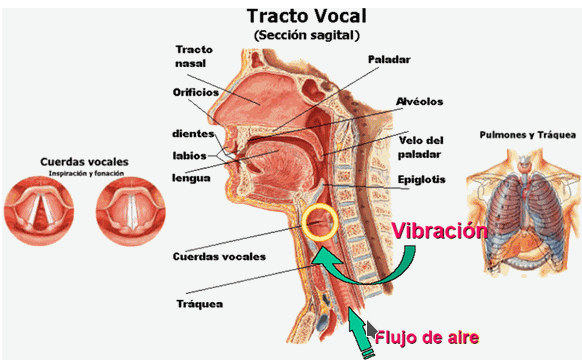
\includegraphics[width=\textwidth]{imagenes/03_02_aparato_fonador.png}
\end{figure}

El Alfabeto Fonético Internacional o IPA por sus siglas en inglés, fue estructurado desde 1888 y representa todas las posibles configuraciones para los fonemas que pueden ser ejecutados por el ser humano y la caracterización e identificación que da a las vocales es la que se puede observar en la tabla \ref{tab:ipa_table_vowels}


% \begin{landscape}
\begin{table}
\centering
\caption{Alfabeto Fonético Internacional: Vocales}
\label{tab:ipa_table_vowels}
\begin{tabular}{|l|l|l|l|l|l|l|}
\hline
{} & \multicolumn{2}{|c|}{Frontal} & \multicolumn{2}{|c|}{Central} & \multicolumn{2}{|c|}{Posterior}   \\
\hline
Cerrada & i  & y &\textbaru   & \textbari & \textturnm &  u  \\
\hline
Casi cerrada & \textsci  & \textscy &  \multicolumn{2}{|c|}{} &  & \textupsilon  \\
\hline
Semicerrada & e  & \textipa{\o} &\textreve &  \textbaro & \textramshorns & o \\
\hline
Intermedia &  \multicolumn{2}{|c|}{} & \multicolumn{2}{|c|}{\textschwa} &  \multicolumn{2}{|c|}{} \\
\hline
Semiabierta &\textepsilon  & \textipa{\oe} & \textrevepsilon & \textcloserevepsilon  & \textturnv & \textopeno \\
\hline
Casi abierta & \multicolumn{2}{|c|}{\ae} &\multicolumn{2}{|c|}{\textturna} &  \multicolumn{2}{|c|}{}  \\
\hline
Abierta & a  & \textscoelig &  \multicolumn{2}{|c|}{}  &\textscripta & \textturnscripta \\
\hline
\end{tabular}
\end{table}
% \end{landscape}

Además de estas alteraciones principales en las perturbaciones del aire, existen otros sonidos que interrumpen el flujo de aire emitido por el diafragma. Estos sonidos son denominados consonantes y son clasificados por su lugar de articulación y el tipo de articulación. El IPA también define una clasificación para las consonantes, la cual puede observarse en la tabla \ref{tab:ipa_table_pulmonic_consonants} y la tabla \ref{tab:ipa_table_non_pulmonic_consonants}

\begin{landscape}
\begin{table}
\centering
\caption{Alfabeto Fonético Internacional: Consonantes pulmónicas}
\label{tab:ipa_table_pulmonic_consonants}
\begin{tabular}{|p{25mm}|l|p{15mm}|l|l|p{15mm}|l|l|l|l|l|l|}
\hline
{} & Bilabial & Labio\newline dental & Dental & Alveolar & Post-\newline alveolar & Retrofleja & Palatal & Velar & Uvular & Faríngea & Glotal \\
\hline
Plosiva& p b  & & \multicolumn{3}{|c|}{t d} & \textipa{\:t \:d } & \textipa{c \*j} & k g &  q G & & \textipa{P} \\
\hline
Nasal& m &  \textipa{M} & \multicolumn{3}{|c|}{n} & \textipa{\:n}  &  \textipa{\*n}  & \textipa{N} & N &  & \\
\hline
Vibrante& B & & \multicolumn{3}{|c|}{r}  & & & & R &  & \\
\hline
Aproximante & & \textipa{v} & \multicolumn{3}{|c|}{\textipa{R}} & \textipa{\:r} & & & & &  \\
\hline
Fricativa  & \textipa{F B}& f v & \textipa{T D} & s z & \textipa{S z} & \textipa{\:s \:z} & \textipa{\c{c} J}& x \textipa{G} &\textipa{X  K}  &\textcrh \textipa{Q} & h\textipa{H}  \\
\hline
Lateral \newline fricative& & & \multicolumn{3}{|c|}{\textbeltl \textipa{\*z}} & & & & &  & \\
\hline
Aproximante & & \textipa{V}& \multicolumn{3}{|c|}{\textipa{\!R}} & \textipa{\:R} & j  & \textturnmrleg & & &  \\
\hline
Aproximante lateral& & \multicolumn{3}{|c|}{\textipa{l}} &  \textraisevibyi & \textturny & \textipa{\;L} & & & & \\
\hline
\end{tabular}
\end{table}
\end{landscape}

% \begin{landscape}
\begin{table}
\centering
\caption{Alfabeto Fonético Internacional: Consonantes no pulmónicas}
\label{tab:ipa_table_non_pulmonic_consonants}
\begin{tabular}{|p{20mm}|l|l|l|l|l|l|}
\hline
{} & Bilabial & Dental & Alveolar  & Palatal & Velar & Uvular   \\
\hline
Eyectiva \newline oclusiva& p\textipa{'}  & &t   & c\textipa{'} & k\textipa{'} &  q\textipa{'}  \\
\hline
Eyectiva \newline fricativa& \textipa{F'}  & \textipa{T'}&  s\textipa{'} & \textipa{\c{c}'} & x\textipa{'} & \textipa{X'}  \\
\hline
Click &\textipa{\!o}  & \textipa{|} & \textipa{!} &  & & \\
\hline
Implosiva & \textipa{\!b}  & \multicolumn{2}{|c|}{\textipa{\!d}} &  \textipa{\!j} & \textipa{\!g} & \textipa{\!G} \\
\hline
\end{tabular}
\end{table}
% \end{landscape}

El español utiliza solamente ciertos fonemas del IPA, y la representación de estos define los conocidos alfabetos fonéticos para el español. Entre los más conocidos se encuentran el SAMPA \cite{SAMPA}, y el Mexbet, el cual se representa en la tabla \ref{tab:mexbet} \cite{mexbet}.

\begin{table}[H]
\centering
\caption{Mexbet}
\label{tab:mexbet}
\begin{tabular}{|l|l|l|l|l|l|l|}
\hline
\textbf{Consonantes}         & \textbf{Labial}     & \textbf{Labio dental} & \textbf{Dental}     & \textbf{Alveolar}    & \textbf{Palatal}    & \textbf{Velar}  \\ \hline
Oclusivos Sordos             & p (p)&       & t (t)&       &       & k (k)\\ \hline
Oclusivos Sonoros            & b (b)&       & d (d)&       &       & g (g)\\ \hline
Africado Sordo               &      &       &      &       & tS (t\textipa{S}) &     \\ \hline
Fricativos Sordos            &      & f (f) &      & s (s) &       & x(x)\\ \hline
Fricativos Sonoros           &      &       &      &       & Z (\textipa{J})&     \\ \hline
Nasales                      & m (m)&       &      & n (n) & n$\sim$ (\textipa{\:n})             &     \\ \hline
Lateral                      &      &       &      & l (l) &                 & \\ \hline
Vibrante                     &      &       &      & r ({\textipa{\!R}})    &                 & \\ \hline
\end{tabular}
\end{table}

Para esto se realizó una anotación fonética manual sobre grabaciones del Open Speech Corpus \cite{Collazos2015} del subcorpus de palabras aisladas, el cual esta compuesto por 334 palabras distintas grabadas por múltiples locutores con un total de 9441 grabaciones de 39 locutores distintos, seleccionando aleatoriamente 100 palabras distintas y realizando una anotación manual por medio de PRAAT \cite{Praat}.

La anotación se realizo utilizando la convención definida en la tabla \ref{tab:anotacion_fonetica}. esta convención se uso considerando que el Open Speech corpus - words fue grabado en su totalidad por locutores latino americanos, del país Colombia y la región del Valle del Cauca. En esta representación fonética, se usa la palabra especial sil para determinar silencio; también se eliminan fonemas como la z fricativa dado que esta forma de pronunciación no es natural de la región de los hablantes.


\begin{table}[H]
\centering
\caption{Anotación Fonética}
\label{tab:anotacion_fonetica}
\begin{tabular}{|l|l|l|}
\textbf{Simbolo} & \textbf{Letra} & \textbf{Representación} \\ \hline
sil              & & Silencio                               \\ \hline
a                & a & vocal open central                   \\ \hline
b                & b &  consonante plosiva bilabial sonora   \\ \hline 
k                & c &  consonante plosiva palatal no sonora \\ \hline 
S                & ch &  consonante fricativa palatal        \\ \hline 
d                & d &  consonante plosiva dental sonora     \\ \hline 
e                & e &  vocal semi-open central              \\ \hline
f                & f &  consonante fricativa labiodental     \\ \hline 
g                & g &  consonante plosiva velar sonora      \\ \hline
i                & i &  vocal closed front                   \\ \hline
j                & j &  consonante approximant palatal       \\ \hline
l                & l &  consonante approximant alveolar      \\ \hline 
m                & m &  consonante nasal bilabial            \\ \hline 
n                & n &  consonante nasal alveolar            \\ \hline 
N                & ñ &  consonante nasal palatal             \\ \hline 
o                & o &  vocal semi-closed back               \\ \hline
p                & p &  consonante plosiva no sonora         \\ \hline 
R                & r &  consonante vibrant alveolar sonora   \\ \hline 
r                & r &  consonante vibrant alveolar no sonora \\ \hline
s                & s &  consonante fricativa alveolar         \\ \hline
t                & t &  consonante plosiva dental no sonora   \\ \hline
u                & u &  vocal closed back                    \\ \hline
y                & y &  consonante fricativa palatal         \\ \hline
\end{tabular}
\end{table}

La distribución de fonemas en la anotación manual se muestra en la tabla \ref{tab:distribucion_fonetica}

\begin{table}[H]
\centering
\caption{Distribución fonética}
\label{tab:distribucion_fonetica}
\begin{tabular}{|l|l|}
\textbf{Fonema} & \textbf{Ocurrencias} \\ \hline
sil & 173 \\ \hline
a   & 91  \\ \hline
o   & 79  \\ \hline
e   & 59  \\ \hline
n   & 45  \\ \hline
i   & 40  \\ \hline
l   & 31  \\ \hline
s   & 29  \\ \hline
t   & 27  \\ \hline
d   & 22  \\ \hline
R   & 22  \\ \hline
b   & 20  \\ \hline
r   & 19  \\ \hline
p   & 19  \\ \hline
j   & 16  \\ \hline
u   & 16  \\ \hline
m   & 15  \\ \hline
k   & 14  \\ \hline
g   & 11  \\ \hline
f   & 7   \\ \hline
c   & 5   \\ \hline
y   & 5   \\ \hline
C   & 2   \\ \hline
N   & 1   \\ \hline
S   & 1   \\ \hline
\end{tabular}
\end{table}

Las grabaciones seleccionadas se distribuyen entre 22 grabadas por locutores de género femenino, 68 masculinos y 10 no identificado.

En la imagen \ref{img:anotacion_fonetica_praat} se muestra la anotación fonética de realizada en Praat y en el archivo \ref{file:text_grid} el archivo correspondiente a la anotación fonética



\begin{figure}[H]
\caption{Anotación fonética con Praat}
\label{img:anotacion_fonetica_praat}
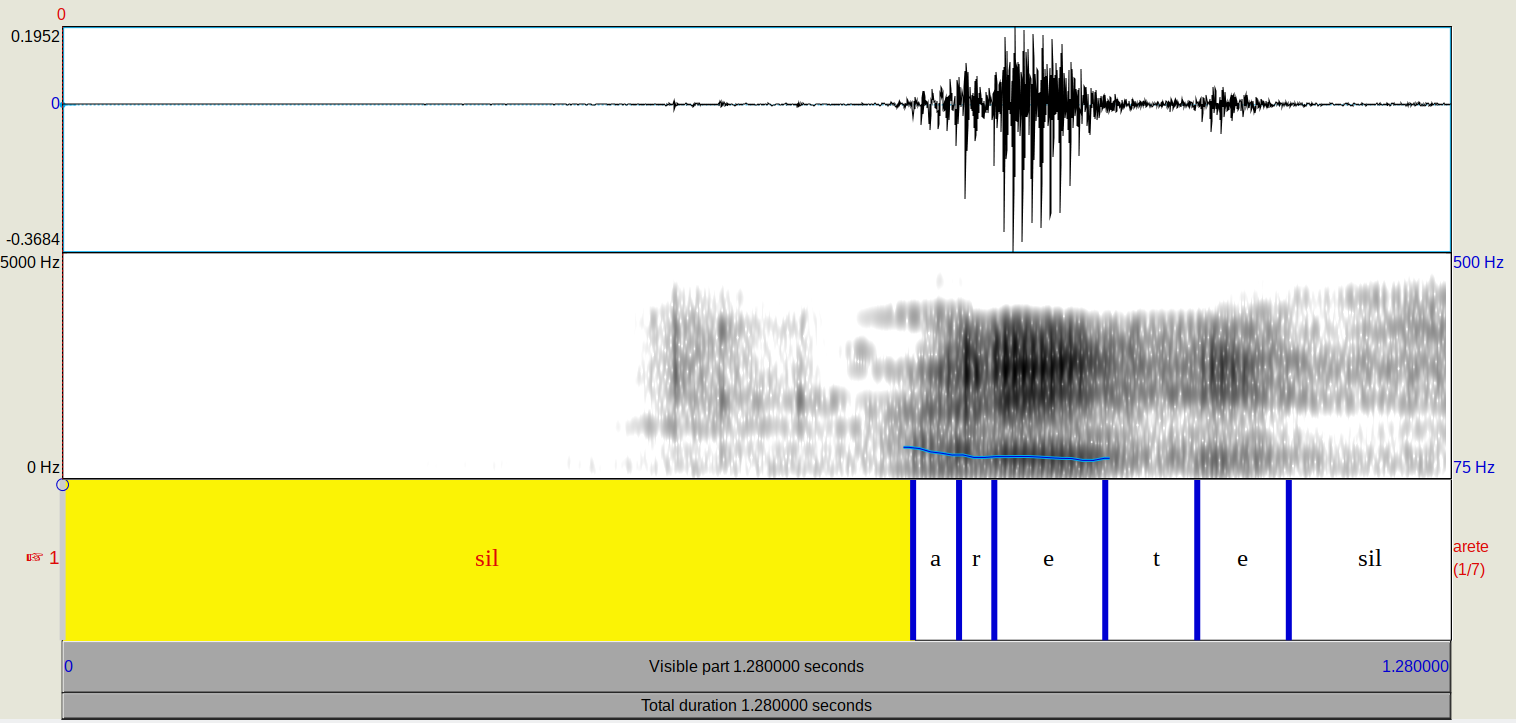
\includegraphics[width=\textwidth]{imagenes/03_01_anotacion_fonetica.png}
\end{figure}

\lstinputlisting[caption={Archivo TextGrid con anotación fonética}, label={file:text_grid}]{archivos/03_01_text_grid_ejemplo.txt}



\section{Anotación manual a nivel de sentencia}

También se realizó una anotación a nivel de declaración de los audiolibros de Librivox, seleccionando audios correspondientes a 6 horas de grabación, sobre los cuales se realizó una segmentación manual basada en símbolos de puntuación.

Para la selección de los audio libros, se ordenaron las grabaciones en orden ascendente considerando el tamaño del audio original en segundos, para posteriormente seleccionar 3 horas de locutores de género femenino y 3 horas del género masculino, garantizando de esta manera un balance de género y también la maximización de locutores diferentes. Cada archivo será identificado con un prefijo F o M que significa el género del locutor, separado por una línea baja \_ y el consecutivo asignado.

Los archivos almacenados en Librivox usan el formato de compresión con pérdida MP3, para su tratamiento son transformados a formato sin compresión WAV utilizando el programa Sox \cite{Sox}.

Se realizó de igual manera una descarga manual de los textos correspondientes a los audio libros seleccionados, generando archivos de texto plano cuya primera línea es el título del texto y el resto del archivo.

Como parte del pre-procesamiento del texto, se utilizaron expresiones regulares para segmentar los textos descargados de internet por símbolos de puntuación, y generando un nuevo archivo de texto plano donde cada línea contiene un índice, y la declaración correspondiente al segmento del texto.

Se muestra un ejemplo de texto tokenizado en el archivo \ref{file:texto_tokenizado}

\lstinputlisting[caption={Texto tokenizado}, label={file:texto_tokenizado}]{archivos/03_02_tokenizacion_texto.txt}

Los índices al comienzo de cada línea funcionan como identificadores en el proceso de anotación a nivel de declaración. Esto con el objetivo de facilitar el proceso de anotación al solo indicar en el campo de texto un índice en lugar del texto correspondiente. Posteriormente es posible reconstruir un archivo de anotación, reemplazando los índices por el texto correspondiente almacenado en el archivo de tokenización. El ejemplo de anotación de declaración del texto ejemplo se puede observar en el archivo \ref{file:text_grid_tokenizado}

\lstinputlisting[caption={Texto tokenizado}, label={file:text_grid_tokenizado}]{archivos/03_03_text_grid_tokenizado.txt}


\section{Anotación automática a nivel de sentencia usando Libri Vox Spanish}

\textcolor{red}{WIP}

Esta sección corresponde a la generación de TextGrids usando los archivos fuentes descargados directamente desde librivox y comparándolos con la segmentación manual de \cite{LibriVox-Spanish}, de momento no tengo nada acá mas que experimentos fallidos usando Onsets y de pronto luego miro si hay tiempo de dejar este capítulo si encuentro alguna luz. De pronto usando DTW pasa algo acá pero no se.



\chapter{Segmentación y Alineación automática}

Como la creación de recursos de manera manual es costosa, y los requerimientos de volúmen de información son altos, la generación automática o semi automática de recursos de habla toma gran relevancia en la investigación actual.

Dado que existen recursos abiertos y disponibles, pero no aptos para la invetigación, el procesamiento de estos de manera automática o semi automática debe garantizar nuevos recursos aptos para la investigación. Las tareas relacionadas con este problema son las de segmentación, la cual toma una señal de audio y extrae segmentos relevantes dentro de esta; la anotación, que toma una señal e identifica componentes de lenguaje dentro de esta y la alineación, que toma una señal e indica los lugares exactos en los cuales existe información de lenguaje.

El problema de la segmentación puede abordarse a nivel de declaración, palabra o fonema, y se presentan dos aproximaciones para realizar segmentación de audios.

\section{Segmentación basada en silencio}

Las segmentación basada en silencio es una respuesta natural al problema de como segmentar señales de voz, pues existe una correspondencia directa entre símbolos de puntuación y pausas en la voz. De igual manera en una señal de voz, los locutores requieren pausas para tomar aire, lo que permite que exista una cadencia en la señal y espacios donde realizar los cortes.

Para identificar el proceso de segmentación por silencios, es necesario entender como se almacenan las señales de voz digitalmente y como se puede procesar este tipo de datos.

La manera mas sencilla de representar digitalmente una señal de voz es haciendo el uso de la Modulación por Impulsos Codificados o PCM por sus siglas en inglés, donde por medio de un transductor análogo, se capturan las variaciones en la presión del aire y se registran como un rango de valores normalizado. El senso de la señal se hace periódicamente a una frecuencia determinada generando de esta manera una secuencia de valores que representa la señal. El proceso de representar la presión del aire en un segmento de tiempo se denomina cuantización, y para señales de audio se utilizan valores normalizados entre -127 y 128 a 16000 Hz de frecuencia.

En al figura \ref{img:pcm} se muestra la visualización de una grabación correspondiente a la palabra agua, en su longitud original y aumentada en un 500\% y 1000\% usando Audacity \cite{audacity}
\begin{figure}[H]
\caption{Representación visual de una señal de voz \cite{hableomsDeVoz}}
\label{img:pcm}
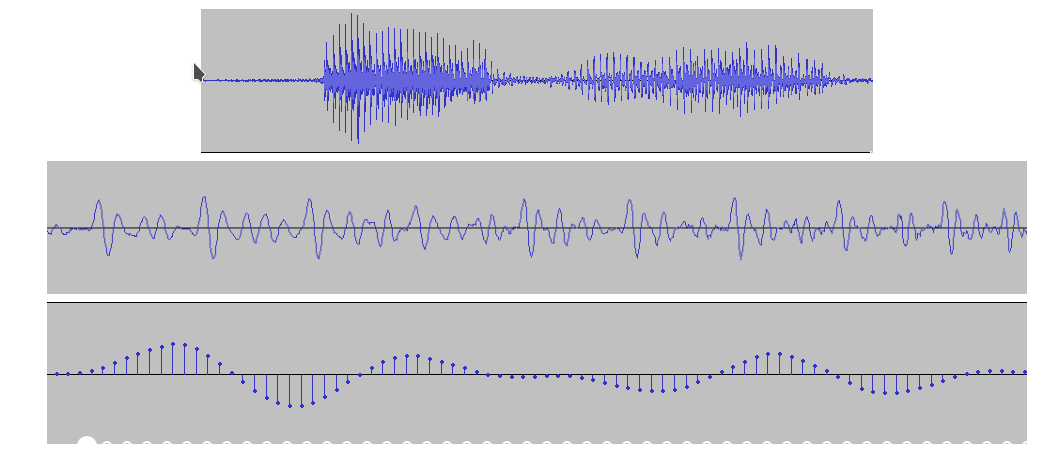
\includegraphics[width=\textwidth]{imagenes/04_01_pcm.png}
\end{figure}

Al hablar de silencio, nos referimos a ausencia total o parcial de sonido, lo cual se puede relacionar directamente con la intensidad de la señal en un segmento de tiempo.

Definiremos intensidad como la sumatoria de las energías en un periodo de tiempo  \cite{Jurafsky2000SpeechRecognition}    

\begin{equation}
\label{eq:energy}
I = \sum{x^2}  
\end{equation}

Esto nos daría un indicador de la toda la señal, sin embargo, es útil realizar este análisis por pequeños segmentos del audio para identificar en conjunto cuales son los puntos donde la intensidad baja representa un espacio de silencio. Estos segmentos por lo general se definen en espacios de 250ms solapados cada 100ms, aunque este solapamiento no es necesario para el proceso de identificación de intensidad, da la idea de que la señal es continua y que cada segmento comparte información con el anterior.

Utilizando esta idea es posible tomar cualquier señal de voz, segmentarla cada 250ms y encontrar los segmentos consecutivos donde la intensidad sea baja o cercana a cero y estos segmentos consecutivos representarían pausas de silencio.

Algunas consideraciones a tomar al usar esta aproximación es que incluso en medio de las señales de voz, existen subsegmentos donde la intensidad es baja, por ejemplo en la pronunciación de consonantes plosivas, como la b, c, d, g, p y t existe una interrupción momentánea y completa del flujo de aire, causando momentáneamente segmentos de silencio.

Usando las anotaciones fonéticas se determinó que la duración promedio de cada consonante plosiva es inferior a los 100ms, también realizando una anotación manual de sonidos y silencios sobre múltiples grabaciones de la anotación por declaración se determinó que los espacios de silencio entre frases eran de mínimo 500ms. De esta manera, utilizando segmentación de 250ms de longitud y desplazamiento de 100ms, se determinan como silencios los conjuntos de segmentos consecutivos de tamaño superior a cinco. 

Entendiendo la condición necesaria para determinar los silencios en una grabación de voz, es posible ejecutar el proceso asumiendo el silencio como ausencia completa de señal, sin embargo, salvo en condiciones muy especiales, donde exista un ambiente libre de ruido, como en un estudio de grabación con filtros físicos, análogos o digitales, en los espacios de silencio la intensidad no es estrictamente cero.

Mas aún, dependiendo de las condiciones y ambiente de grabación, los valores de intensidad en segmentos de silencio varían.

Considerando esto, se propusieron dos aproximaciones para determinar los segmentos de silencio, la primera normalizando los valores de la señal y definiendo un umbral fijo de intensidad en proporción al valor mas alto de la grabación, considerando valores de 0.3, 0.15 y 0.15 que representan umbrales de intensidad del 30\%, 15\%, y 5\%. También se experimentó utilizando algoritmos de agrupamiento con dos centroides iniciales en 0 y la intensidad máxima.

Los resultados se presentan en la tabla \ref{tab:resultados_segmentacion_silencios}

\begin{table}[H]
\centering
\caption{Resultados de la segmentación por silencios}
% \caption{Speech English Corpus}
\label{tab:resultados_segmentacion_silencios}
\begin{tabular}{|l|l|}
\hline
\textbf{Umbral} & \textbf{Precisión}  \\ \hline
Fijo 30\%       & 57.01\%             \\  \hline
Fija 15\%       & 83.26\%             \\  \hline
Fija 5\%        & 69.05\%             \\  \hline
Dinámico        & 74.53\%             \\  \hline
\end{tabular}
\end{table}


\section{Alineación basada en duración de fonemas}

\textcolor{red}{WIP}

Utilizando la segmentación basada en silencios, para determinar cuales son los textos correspondientes se realiza una alineación basada en la duración estimada de un segmento de texto y la duración de los segmentos calculados. Para esto se tomó la anotación fonética para determinar la duración promedio y la desviación estándar de la duración de cada fonema.

Dicha información se puede ver en la tabla \ref{tab:duracion_promedio_fonemas}

\begin{table}[H]
\centering
\caption{Distribución fonética}
\label{tab:duracion_promedio_fonemas}
\begin{tabular}{|l|l|l|}
\textbf{Fonema} &\multicolumn{1}{|p{2cm}|}{\textbf{Duración promedio}} & \multicolumn{1}{|p{2cm}|}{\textbf{Desviación estándar}} \\ \hline
sil & 0.6619 & 0.3700 \\ \hline
a   & 0.1421 & 0.0566 \\ \hline
o   & 0.1487 & 0.0607 \\ \hline
e   & 0.1204 & 0.0416 \\ \hline
n   & 0.1090 & 0.0442 \\ \hline
i   & 0.1294 & 0.0404 \\ \hline
l   & 0.1125 & 0.0530 \\ \hline
s   & 0.1811 & 0.1059 \\ \hline
t   & 0.0784 & 0.0507 \\ \hline
d   & 0.0877 & 0.0536 \\ \hline
R   & 0.0999 & 0.0517 \\ \hline
b   & 0.0826 & 0.0610 \\ \hline
r   & 0.0750 & 0.0254 \\ \hline
p   & 0.0692 & 0.0649 \\ \hline
j   & 0.1038 & 0.0659 \\ \hline
u   & 0.1441 & 0.0507 \\ \hline
m   & 0.1183 & 0.0515 \\ \hline
k   & 0.1224 & 0.0904 \\ \hline
g   & 0.1016 & 0.0970 \\ \hline
f   & 0.1402 & 0.0569  \\ \hline
c   & 0.1032 & 0.0838  \\ \hline
y   & 0.1118 & 0.0044  \\ \hline
C   & 0.1274 & 0.0248  \\ \hline
N   & 0.0575 & 0  \\ \hline
S   & 0.0927 & 0  \\ \hline
\end{tabular}
\end{table}

\section{Segmentación basada en información fonética de formantes en vocales}

Base teórica de los formantes 1 y 2 para vocales en español

Cálculo observado para formantes 

Gráfica de formante promedio +- desviación estandar sobre grabación vocálica

\addcontentsline{toc}{chapter}{Bibliography}
\bibliographystyle{plain}
% \bibliographystyle{apacite}
% \bibliography{bibliography/bibliography}
\bibliography{referencias_ante_proyecto.bib,custom_references_ante_proyecto.bib,references_chapter_1.bib}

\end{document}
